% !TeX spellcheck = de_DE_frami
\documentclass[11pt, a4paper, twoside, bibliography=totoc]{scrartcl}

\usepackage{fontspec}
\usepackage{polyglossia}
\setmainlanguage[variant=british]{english}
\setlength{\parindent}{0pt} % we don't want paragraph indettaion  

\usepackage{amssymb}
\usepackage{amsfonts}
\usepackage{amsmath}
\usepackage{enumerate}

\usepackage{booktabs}
\usepackage{graphicx}
\usepackage[xetex]{geometry}
\usepackage{scrlayer-scrpage}
\usepackage{multicol}
\usepackage{color}
\usepackage{makeidx}
%\usepackage{lineno}

\usepackage{wrapfig}
\usepackage{subfig}
\usepackage{bibgerm}
\usepackage{textcomp}
\usepackage[xetex,
            bookmarksopen=true,
            hyperfootnotes=false,
            breaklinks=true,
            bookmarks=false,
            pdfpagemode=UseOutlines,
            pdftitle={An Introduction to Coq},  
            pdfauthor={Tanja Almerothh},
            pdfcreator={Steffen Reith}
           ]{hyperref}
\hypersetup{colorlinks=true,citecolor=blue,linkcolor=blue,urlcolor=blue}
\usepackage{hypcap}
\usepackage[numbered]{bookmark}
\usepackage{microtype} % some formatting
\usepackage{script}
%\usepackage{myMakros}
\usepackage{caption}
\usepackage{import}
\usepackage[toc]{glossaries}


\usepackage{listings}
\usepackage{lstcoq}
\lstset{language=coq, % Coq
		tabsize=4, % Tabulatorbreite
		linewidth=\linewidth, % Width of a line
		breaklines=true, % Break long lines
		breakatwhitespace=true, % Only break at whitespaces
		basicstyle=\scriptsize\ttfamily, % Schriftart/-größe
		numbers=left, % Linenumbers left
		numberfirstline=false, % Not: Always number 1. line
		numberstyle=\scriptsize, % Größe der Zeilennummern
		stepnumber=1, % Jede 2. Zeilennummer anzeigen
		numbersep=5pt, % Abstand Nr - Quellcode
		showspaces=false, % Spaces nicht anzeigen
		showtabs=false, % Tabs nicht anzeigen
		showstringspaces=false, % Don't show tabs in strings
		showlines=false, % Leerzeilen am Sourceende weglassen
		extendedchars=true, % ASCII-Zeichnen > 127 zulassen
		identifierstyle=\bfseries, % Identifier
		keywordstyle=\bfseries, % Keywords
		commentstyle=\itshape, % Style of comments
		stringstyle=\ttfamily, % Strings (!= Keywords)
		flexiblecolumns=false, % Use fixed width for fonts
		fontadjust=true, % "Base width" nicht jede Zeile anpassen
		frame=trbl, % Frame; trBL
		captionpos=b, % Position of the caption
		aboveskip=25pt}% Space between text and the top of the listing


% Algorithmen in C-Style
%\SetKwIF{If}{ElseIf}{Else}{if}{\{}{\}\\else if }{\}\\else\{}{\}}%
%\SetKwSwitch{Switch}{Case}{Other}{switch}{\{}{case}{default:}{\}}%
%\SetKwRepeat{Repeat}{do \{}{\} while}%
%\SetKwBlock{Begin}{\{}{\}}
%\SetKwFor{For}{for}{\{}{\}}
%\SetKwFor{While}{while}{\{}{\}}
%\SetKwInput{KwData}{Eingabe}
%\SetKwInput{KwResult}{Ergebnis}
%\renewcommand{\listalgorithmcfname}{Algorithmenverzeichnis}%

% Baue einen Index
\makeindex

% Bause ein Glossar
\makeglossaries

% Include global settings
% Special settings for discrete mathematics
\newif\ifdiscretemath
\discretemathfalse

\discretemathfalse
\algorithmsfalse
\komplextrue

% Baue einen Index
\makeindex

% Setze bibliography style
\bibliographystyle{alpha}

% Seitenaufteilung
\geometry{top=2.5cm, left=3.25cm, right=3.25cm, bottom=3.0cm}

% Suchpfad fuer Graphiken
\graphicspath{{pics/}}

%scrlayer-scrpage
\automark[subsection]{section}
\lofoot[]{}
\cofoot[]{\pagemark}
\rofoot[]{}
\refoot[]{}
\cefoot[]{\pagemark}
\lefoot[]{}

% Definitionen für die Titelseite
\newcommand{\docutyp}{Skript}
\newcommand{\lecture}{An Introduction to Coq}
%\newcommand{\docudate}{Wintersemester 2018/2019}
\newcommand{\docudate}{Sommersemester 2019}

\newcommand{\institution}{{\Large Hochschule RheinMain}\\
                          Fachbereich Design Informatik Medien}
\newcommand{\lecturer}{Tanja Almeroth}
\newcommand{\lectureremail}{\href{mailto:tanja.almeroth@hs-rm.de}{tanja.almeroth@hs-rm.de}}

\newcommand{\writer}{Tanja Almeroth}
\newcommand{\reviser}{xxx xxx}
\newcommand{\email}{Tanja.Almeroth@hs-rm.de}
\newcommand{\writtendate}{Mai 2019}

\begin{document}

\pagestyle{scrplain}

\begin{titlepage}

        \vspace{40pt}
	\begin{center}

                
		\vspace{20pt}
		\textbf{\Large {\docutyp}}
			
		\vspace{20pt}
		\textbf{\Huge \lecture}
			
		\vspace{20pt}
		\textbf{\docudate}

		\vspace{20pt}
		\textbf{\lecturer}\\
		\textbf{\lectureremail}
		
		\vspace{120pt}
		{\institution}\\
		
		\vfill			
		\vspace{20pt}
		
	\end{center}
	\newpage
\end{titlepage}

\cleardoublepage

\vspace{0.3\textheight} 
%\begin{raggedleft}
%Wenn Leute nicht glauben, dass Mathematik\\
%einfach ist, dann nur deshalb, weil sie nicht begreifen,\\
%wie kompliziert das Leben ist.\\[\smallskipamount]
%\hfill \textsc{John von Neumann}%
%\end{raggedleft}

\vspace*{1.5cm}

%\begin{raggedleft}
%Wenn es eine gute Idee ist, dann mach es\\ 
%einfach. Es ist viel einfacher sich hinterher zu\\
%entschuldigen, als vorher dafür eine\\
%Genehmigung zu bekommen.\\[\smallskipamount]
%\hfill \textsc{Grace Hopper}%
%\end{raggedleft}

\vspace*{1.5cm}
%
%\begin{raggedleft}
%Wake up! Time to die!\\[\smallskipamount]
%\hfill \textsc{Leon} in Blade Runner%
%\end{raggedleft}

\vfill

%Dieses Skript ist aus den Fragen und Bemerkungen von Studenten des
%Diplom, Bachelor und Master-Studiengangs Informatik an der Hochschule
%RheinMain (ehemals Fachhochschule Wiesbaden) hervorgegangen. Ich danke
%allen meinen Studenten für konstruktive Anmerkungen und
%Verbesserungen. Dabei möchte ich besonders Frau Carola Henzel nennen,
%die sehr viele Tippfehler (Mengen, Summen und Beweistechniken)
%berichtigte. Herr Kim Stebel hat die Bemerkungen zu bipartiten Graphen
%verbessert. Herr Norbert Wesp berichtete über sprachliche Fehler in
%Abschnitt \ref{sec:proof} und Tippfehler in der Einleitung. Eine größere 
%Anzahl von Tipp- und Flüchtigkeitsfehlern wurden von Herrn Marcell Dietl
%entdeckt und gemeldet. Danke!
%
%Naturgemäß ist ein Skript nie fehlerfrei (ganz im Gegenteil!) und es
%ändert (mit Sicherheit!) sich im Laufe der Zeit. Es sollte Ihnen klar 
%sein, dass Fehler, Ungenauigkeiten und Unklarheiten natürlich nur 
%aus didaktischen Gründen und zu Ihrer  Belustigung eingebaut 
%wurden. Finden Sie diese Fehler und verbessern Sie mich!

\cleardoublepage

\tableofcontents

\cleardoublepage

% Seitenstil (Fuss- und Kopfzeilen)
\pagestyle{scrheadings}

\pagenumbering{arabic}
	
%%%%%%%%%%%%%%%%%%%%%%%%% content begin %%%%%%%%%%%%%%%%%%%%%%%%%%%

% glossary entries

% example:
%\newglossaryentry{foo}{name={foo},description={},see={bar,baz}}
%\setabbreviationstyle[acronym]{long-short}
%\newacronym{laser}{laser}{light amplification by stimulatedemission of radiation}

\newglossaryentry{Isabelle}{
	name = Isabelle,
	description = {A generic proof assitant \url{https://isabelle.in.tum.de/} }
}

\newglossaryentry{CoC}{
	name = Calculus of Constructions,
	description = {´´The calculus of constructive proofs is a natural deduction style.''
	 	\url{https://doi.org/10.1016/0890-5401(88)90005-3}}
}

\newglossaryentry{Hadoop}{
	name = Hadoop,
	description = {open-source software project for relaiblae, scalable und distrubuted computing.
	\url{https://hadoop.apache.org} }
}

\newglossaryentry{Emacs}{
	name = Emacs,
	description = { a text editor
}}

\newglossaryentry{SAT-solver}{
	name = SAT-solver,
	description = {An algorithm to solve a Boolean satisfubility problem called SAT},
	plural = {SAT-solver},
}

\newglossaryentry{SMT-solver}{
	name = SMT-solver,
	description = {An algorithm solving the SMT-problem, which is determining if a fomula of first order Logic is staisfiable.},
 	plural = {SMT-solvers},
}

\newglossaryentry{model checker}{
	name = model checker,
	description = {Checking weather a model meets a given specification.}
	plural = {model-checkers}
}

\newglossaryentry{coqtop}{	
	name = coqtop, 
	description = {The Coq Proof Assitant top level system \url{https://coq.inria.fr/refman/practical-tools/coq-commands.html}}
}


%TODO:

%standard library

%Boolean 
%Numbers

%data structs

%hash tables

%module

\newglossaryentry{real-time system}{
	name = real-time-system,
	description = { \begin{quote}
	The timing constraint of a task can be hard or soft, depending on weather a rigorous validation of the timing constrained is required (hard) or not (soft).
	In practise a {\itshape hard real-time system invariably} has many {\itshape soft real-time jobs} and vice versa. 
	The deviation is not always as obvious as we made it out to be here and, moreover, is not always necessary. 
	In {\itshape real-time system} or {\itshape system} whenever we mean either {\itshape a hard-real time system} or a {\itshape soft real-time} system or when there is no ambiguity about which type of system is meant by it.
	\end{quote} \cite[chp. 2.6]{L}}
	plural = {real-time systems} 
}
 

\clearpage

% Eine kurze Einleitung
\section{Introduction}

This is a summary of the electronic text-book \cite{PACGGHSY} with comments and a little rewritten sections by the author and based on the peers and supervisor's feedback. 
Other refrences are marked. 
This summary aims to be give a clear instruction of the usage and applicability of Coq.\\

\subsection{Preface}

Within this introduction the mathematical underpinning of reliable software is given the building blocks are
\begin{itemize}
\item basics concepts of logic (see sec. \ref{} % TODO:)
\item computer assisted theorem proving (see sec. \ref{} %TODO:)
\item Coq-proof assistant (see sec. \ref{} %TODO:
\item functional programming (see sec. \ref{} %TODO)
\item operational semantics (see sec. \ref{} %TODO:)
\item logics for reasoning about programs (see sec. \ref{} %TODO: )
\item static type systems (see sec. \ref{} %TODO:)
\end{itemize} 


\subsection{Overview}

There is a lot of motivation for reliable software. 
First of all the scale, complexity and number of involved people in modern systems is increasing.
Therefore building correct software is extremely difficult.
Information processing is waved into every aspect of society, leading to ammplifed costs of bugs and insecurities upto multiple levels.\\
Computer scientists and software engineers have responded to improve reliability with a lot of design threats and to improve reliability and mathematical technices for reasoning.
Within this work it should be contributed to validates these properties. They are:
\begin{enumerate}
\item basic tools from logic for making and justifying precise claims about programs
\item use of proof assistants to construct rigorous logical arguments
\item functional programmings as method of programming and simplifying reasoning about programs as a bridge between programming and logic
\end{enumerate}



\subsection{Logic}

\begin{quote}
``As a matter of fact, logic has turned out to be significantly more effective in computer science then it has been in mathematics.''
\end{quote}
Volumes have been written about the central role of logic in computer science. 
It's fundamental tool {\itshape inductive proof} is going to be explored very deeply within this work.


\subsection{Proof Assistants}

In computer science proof assistants are an important tool for helping construct formal proofs of logical propositions.
There are two categories of these tools.\\
First of all there are automated theorem proofers. 
These are able of a ''push-button- operation'' which returns true, false'' or ``ran out of time'' given a proposition.
Example applications are \gls{SAT-solvers}, \gls{SMT-solvers} or \glspl{model checker}. 
Second there are proof assistants, which are hybrid tools that automate the more routine-like aspects of a proof, while depending on human guidance. 
Examples are \gls{Isabelle}, Agda, Twelf, ACL2, PVS or Coq.\\
The Coq proof assistant has been developed since 1983 and gathered a large community in research and the industry.
It provides a rich environment for interactive development of machine-checked code for formal reasoning.\\
It's kernel is a simple proof checker, ensuring that correct deution of sets are ever performed. 
Moreover, there are high-level facilities for proof development.
Coq has been applied as critical enabler across computer science and mathematics a plattform for modelling programming languages and as an environment for developing {\itshape formally certifed software and hardware}.
 

\subsection{Trivia}

Some French computer scientist have a tradition of naming their software as animal species.
{\itshape Coq} is the French word for roster.
The roster is the national symbol of the French.
Coq sounds like the initial of the \gls{CoC}.
One of Coq's early developers is called Terry Coquand.


\subsection{Functional Programming}

There are two meanings of the term. 
It is either refereed to programming idioms (something like a pattern) or something else as in this work.\\

Functional programming refers to a programming, which is free of side effects.
By side effects phenomena as I/O or redirecting pointers are meant. 
For example, let's imagine iterative sorting. 
A sorting-function might take a list of numbers to and rearrange the pointers to these numbers.
In functional programming a new list is returned which contains the same number arranged in an order.\\ 
Advantages of functional programming are  that we are having a new data structure leaving the old one in tact. 
Therefore there is no reason to worry about the structure being shared, weather one part of the program might break an invariant that another part of the program relies on.\par
The industry is interested in functional programming due to it's simple behaviour in the presence of accuracy.
Furthermore, functional programming is more easy to parallelize then the counter parts.
E.g. the \gls{map-reduce idiom}, which relies at the heart of massively distributed query processor like \gls{Hadoop} is functional programming. 

\begin{quote}
`` [...] When we come to look more closely, we find that these two sides of Coq are actually aspects of the very same underlying machinery - i.e. proofs are programs.'' 
\end{quote}




\subsection{System Requirements}

Coq runs on Windows, Linux and macOS.
A current installation can be found on the Coq-homepage. 
The listings in this work from \cite{PACGGHSY} have been tested using Coq 8.8.1.
The following choices of IDEs are available. 


\paragraph{Coq in the command line}

It is not recommended to use Coq in the command line mode. 
Because the interactive mode is preferred, when using Coq as a proof assistant. 


\paragraph{Proof General}

Proof general is an Emacs based IDE. 
It is recommended to users who are familiar with the Emacs-editor.

\paragraph{CoqIDE}

CoqIDE is a simple stand-alone IDE. 
It should be available with any Coq-installation. 
It shall be warned that CoqIDE should be run with the asynchronous and error reliance model disabled. 

\paragraph{Coquille}

refernces see the CoqIDE documentation.
Coquille is a vim plugin used by the author.
It can be found here: \url{https://github.com/Werner2005/coquille}.
It provides syntax check by color highlighting and and interactive evaluation.  
The author worked with coquille to explorer Coq.\\
It provides a similar workflow as CoqIDE. 
Coquille labels itself as a user friendly  replacement of \gls{coqtop}. 
The running buffer is the one where navigation takes place. 
To that coquille provides forwards and backwards navigation.\\


In order to launch coquille open a Coq script (a \texttt{.v}-file) by gvim or vim from the console and run (\texttt{:CoqLaunch}). 
Coqille's main screen provides an evaluation of the Coq-code untill the position of the curser (press \texttt{F4}), a stepwise forward (press \texttt{F2}) and backwards (press \texttt{F3}) evaluation.                 
Furthermore, the plugin provides syntax highliting (see figure \ref{fig:Coquille}).
While running a buffer it is deposited grey.
A green deposition indicates a correct evaluation. 
And a just prooven subgoals is displayed in the goal window. 
Failing commands are desposited red and the message window reports errors.

 %%%%%%%%%%%%%%%%%%%%%% TODO %%%%%%%%%%%%%%%%%%%%%
\paragraph{Encoding}
Look this up here:Zeichensatz (ASC II)\\
https://coq.inria.fr/refman/language/gallina-specification-language.html
%%%%%%%%%%%%%%%%%%%%%% TODO end %%%%%%%%%%%%%%%%%

\begin{figure}[h]
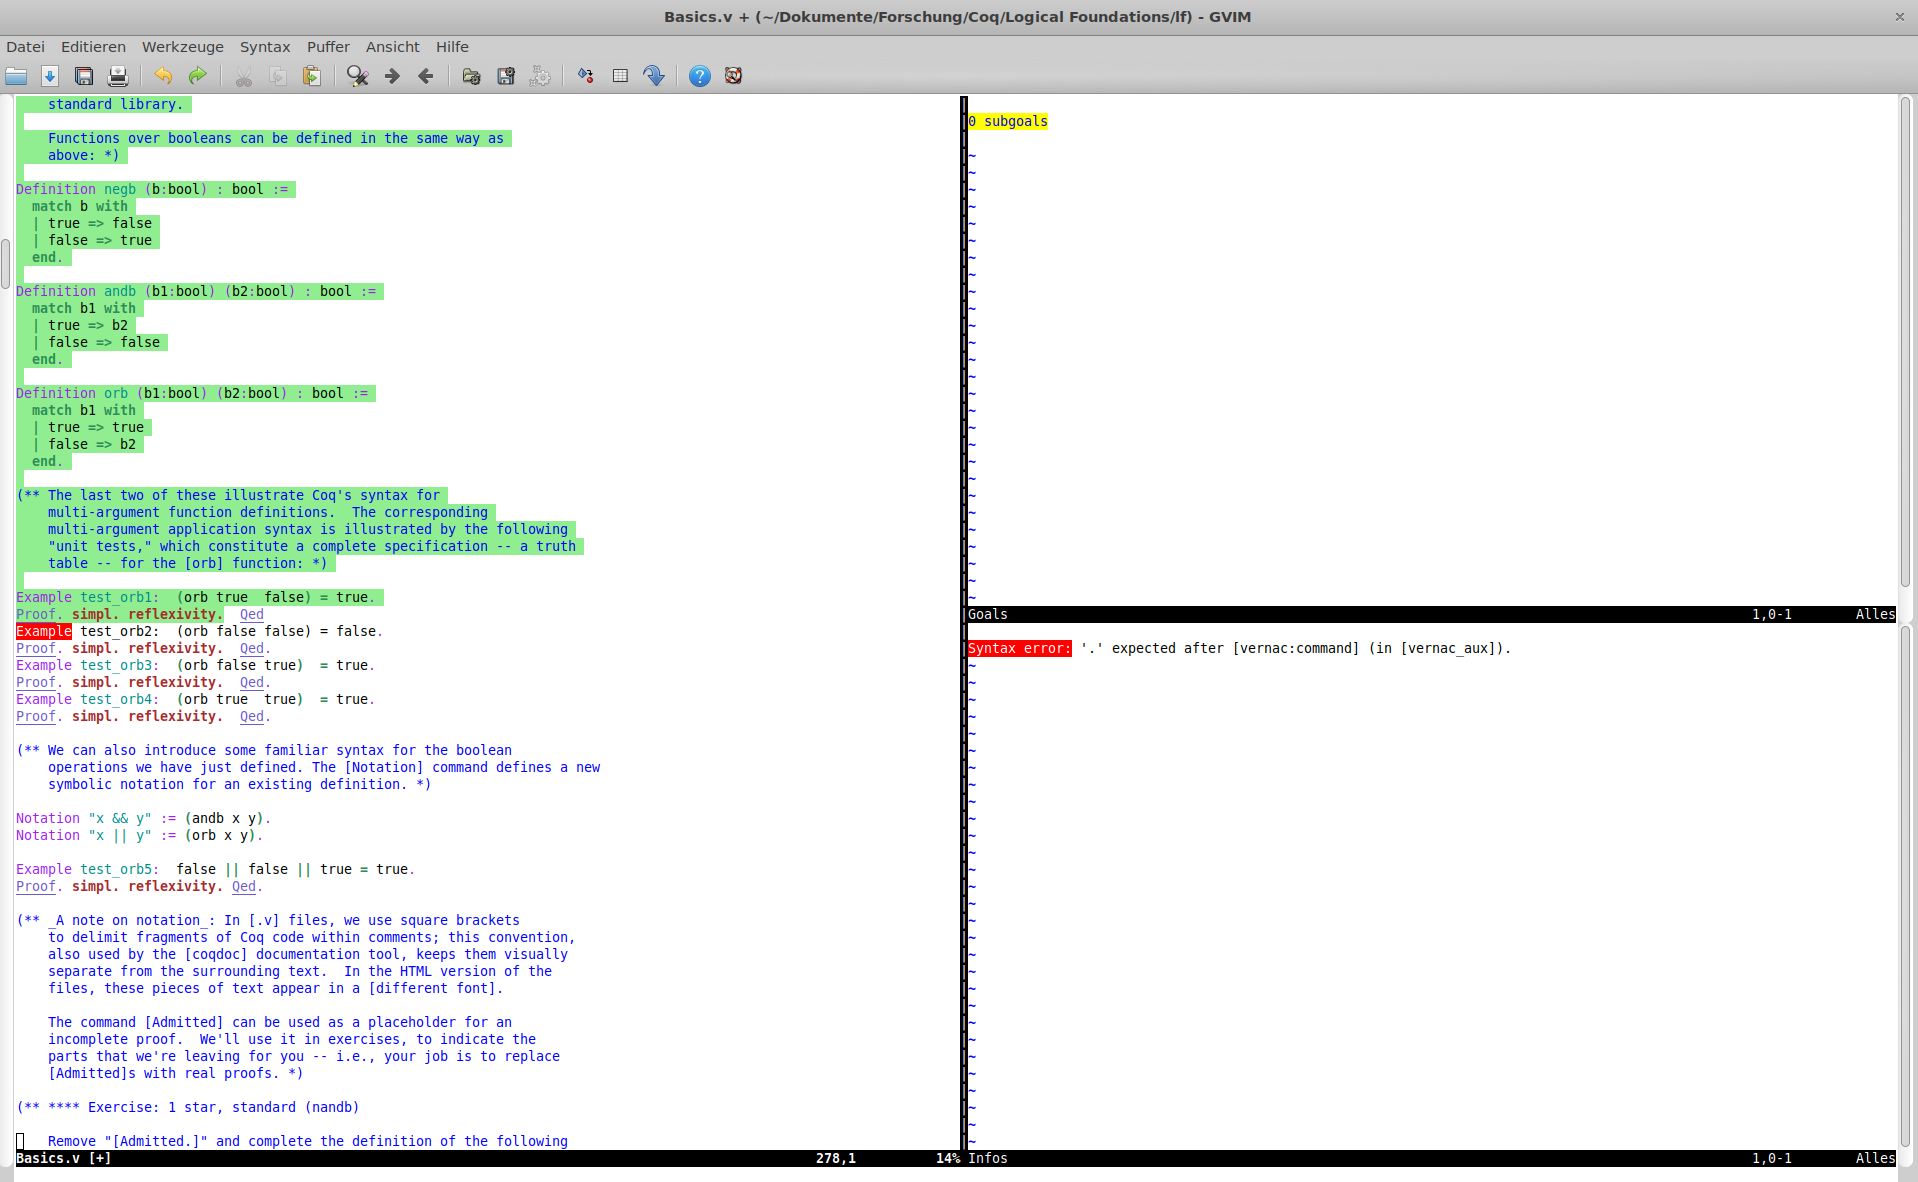
\includegraphics[width=0.9\textwidth]{CoqIDE.png}
\caption{Coq interface launched in gvim using coquille.\\ 
Left window: The open Coq-script \texttt{Basics.v}.
Upper right: The {\itshape goal window}. 
Lower right: The {\itshape message window}.}
\label{fig:Coquille}
\end{figure}

\subsection{Languages}
Coq uses three differnt languages. 
First, there is a vernucular language. 
It is a top-level interaction. 
It's keywords start with a capital letter e.g. \lstinline!Theorem!, \lstinline!Proof! and  \lstinline!Qed!. 
There is the tactics language (e.g. \lstinline!intros! and \lstinline!exact!).
And finally there is an unnamed language of Coq-terms. 
It consits of a lot of operators (e.g. \lstinline!for all A:Prop, A -> A!).
Technically, it is part of the tactics language, but it is useful to think of it as it's own thing.

\cleardoublepage

% Kapitel mit Inhalt

\cleardoublepage

\section{Basic Functional Programming in Coq}



\subsection{Introduction}

In this chapter we are going to introduce the most essential elements of Coq's functional programming language called {\itshape  Gallina}. 
Moreover, {\itshape tactics}, which can be applied to prove properties of Coq programs, are introduced.


\subsection{Data and Functions}

 \paragraph{Enumerated Type}
 
  The built-in features set in Coq is extremely small. In particular, Coq is a powerful mechanism for defining data types from scratch.
  Current Coq distributions come preloaded with an extensive standard library.
  Boolean, numbers, data struts like lists and hash tables.\\
  In this course we are going to explicitly recapitulate the used definitions.
   
  
  \begin{example}
  We are defining a type called \lstinline!day!.
  \begin{lstlisting}
    Inductive day: Type :=
	  | monday
	  | tuesday
	  | wednesday
	  | thursday
	  | friday.
	  | saturday.
	  | sunday.
	  \end{lstlisting} 
  
  The type members are called \lstinline!monday!, \lstinline!tuesday! , \lstinline!wednesday! \ldots{} and \lstinline!sunday!.\\
  
  We are defining a function operating on \lstinline!day!: 
  \begin{lstlisting}
  Definition next_weekday(d:day) day:=
    match d with 
	  | monday => tuesday
	  | tuesday => wednesday
	  | wednesday => thursday
	  | thursday => friday
	  | friday => monday
	  | saturday => monday
	  | sunday => monday.
    end.  
  \end{lstlisting}
  \end{example}

  Coq is able of {\itshape type  interference}, whenever the type is not defined explicitly.
  But for readability, we are including types in the following.
   
  For testing the above definition and function we have three possibilities in Coq:
     
   \begin{enumerate}
   \item Compute a compound expression including the function:\\
 		 \lstinline! compute (next_weekday friday).  (* = monday : day *)! or \\
   		 \lstinline! compute (next_weekday (next_weekday saturday)). (* = tuesday : day *)!
   \item Record an expected behaviour as a Coq-\lstinline!Example! and verify the assertion: 
         E.g.: {\itshape The second weekday after Saturday is Tuesday.}  
   
		   \begin{lstlisting}
		   		Example. test_next_weekday: (next_weekday (next_weeekday(saturday)) = tuesday 
		   		proof. simpl. reflexivity. Qed.
		   \end{lstlisting}
   			The details of the implementation are not important right now. We are going to come back to them later.
   \end{enumerate}   

    Moreover, Coq can be asked to \lstinline!extract! a program from our \lstinline! Definition! in a programming language, which is more conventional, being equipped with a high performance compiler.
    In particular this is one of the main uses of Coq. 
    It provides a method to transfer proved-correct algorithms in Gallina to efficient machine code.
    (Assuming the correctness of the corresponding high performance compile e.g. the Ocaml, Haskell or Scheme compiler. 


\subsection{Booleans}

    Of course, Coq provides an default implementation of Booleans.
    (See the \href{https://www.cs.princeton.edu/courses/archive/fall07/cos595/stdlib/html/Coq.Init.Datatypes.html}{Coq.Init.Datatypes in the Coq-Library documentation}).  
    In the following we are going to be consistent with the Coq library documentation according to the standard library.
    We are going to introduce coinciding selfdefined data types whenever possible.
    Booleans can be defined as follows:
    
    \label{Def:booleans}
    \begin{lstlisting}    
    Inductive bool: Type :=
      | true
      | false.
    \end{lstlisting}
    
    A function with multiple input arguments is implemented by
    \begin{lstlisting}
    Definition orb (b1: bool) (b2: bool) : bool :=
    match b1 with
	  | true -> true
	  | false -> b2
    end.
    \end{lstlisting}
    
    The functions \lstinline!negb! and \lstinline!andb! corresponding to the boolean functions {\emph negation} and {\emph and} are implemented in a similar manner.
     
    And a new symbolic notations is implemented as follows
    \begin{lstlisting}
    Notation "x && y" := (andb x y).
    Notation "x||y" := (orb x y).
    \end{lstlisting}
    
     
\subsection{Notation}
    As in the Coq doc documentation tool the following notation convention is introduced:
     
    \begin{enumerate}
     \item In \texttt{.v-files} comments are annotated by \lstinline!(* some comment *)!. 
     \item Within these comments Coq-code is denoted by \lstinline![example].! 
     \item And we write \lstinline! Admitted.! at the end of an incomplete proof.    
     \end{enumerate}
     
     
\subsection{Types}
     Every expression in Coq has a type.
     \begin{enumerate}
      \item  \lstinline* Check true.* gives the type of the expression \lstinline! boolean!.
      \item \lstinline! Check negb.! returns \lstinline! bool -> bool! . (Read as  ``bool arrow bool'').
              It is the functions input data type and the output data type, given input data of that type.
       \item \lstinline! andb! returns \lstinline!bool->bool->bool!. This function produces an output of type \lstinline! bool! given two inputs of type \lstinline! bool!.
     \end{enumerate}
   
\subsection{New Types from Old}
     
     
	 Note that so far the data-types we have seen were enumerated types.
	 Let's define a data type \lstinline!rgb! and a data type, whose constructor takes this type as an argument.
	\begin{lstlisting}
	 Inductive rgb: Type:=
	  | red     (* These are *)
	  | green   (* the expressions *)
	  | blue.   (* in the set [rgb]. *)
	 \end{lstlisting}
	 The constructors of the type \lstinline!rgb! are \lstinline!red, green! and \lstinline!blue!. 
	 
	 \begin{lstlisting}
	 Inductive color: Type := 
	  | black
	  | white
	  | primary (p:rgb). (* If [p] is in the set [rgb], then the constructor [primary] applied to the argument [p] is an expression in the set color.*) 
	 \end{lstlisting}
	 
	 The expressions in the set color are \lstinline!black, white! and \lstinline!primary!.
	 Note that, expressions formed as above are the only ones belonging to the sets \lstinline!rgb! and \lstinline!color!.
	 

\subsection{Tuples}

    A single constructor with multiple parameters can be used to create a type \lstinline! tuple!.
	\begin{example}[A nybble: half a byte]~\\\vspace{-10mm}
 	 	\begin{lstlisting}
 	 		Inductive bit: Type := (*a bit*) 
 	 		 |B0
 	 		 |B1.
 		    Inductive nybble: Type := (*a nybble*)
 		   	 |bits( b0 b1 b2 b3: bit).
 		   			 	
 		   	Check(bits B1 B0 B1 B0) (* => bits B1 B0 B1 B0 : nybble *)
 		\end{lstlisting}
 		Hence, a tuple of four bits is a nybble.
 		
 		Assume we would like to test a nybble in order to see if all its bits are 0. We are unwrapping the nybble by pattern-matching:
 		\begin{lstlisting}
 		Definition all_zero(nb: nybble): bool :=
 		  match nb with
 	  	    |(bits B0 B0 B0 B0) -> true
 		    |(bits _ _ _ _) -> false (* This wildcard pattern was included to avoid inventing variable names, which are not going to be used. *) 
 		  end.
 		 \end{lstlisting}
 	\end{example}
 	

\subsection{Modules}

	Coq provides a {\itshape module system} to aid organizing large developments.
	In this course most of it is not going to be needed.

	\begin{lstlisting}
	Module X 
	...
	End X
	\end{lstlisting}

\subsection{Numbers}

  Note that on the one hand the types day, bool, bits and tuples have a finite set of values, while on the other hand the set of natural numbers $\mathbb{N}$ is an infinite set.
 
  Hence, we have to construct $\mathbb{N}$ using a data type with a final number of constructors. 
  Recall, many representations of $\mathbb{N}$ exits (e.g. hexadecimal with base 16, octa with base 8, binary with base 2).
  The most familiar might be the decimal representation.\\
  However, each representation of $\mathbb{N}$ can be useful under different circumstances. 
  The binary representation is valuable in computer hardware, because it presents a simple circuitry.
  Here we are aiming to make proofs simple using the unary (base 1) representation.
  
  \begin{lstlisting}
  Module NatPlayground
  Inductive nat: Type :=
    | 0
    | S (n:nat).
  \end{lstlisting}
  
  One might picture this representation by scratches on a wall in prison. \\
  It uses two constructors: 
  \begin{itemize}
  \item The letter \lstinline!0! represents the natural number zero. 
  \item The letter \lstinline!S! represents a natural number $n\in\mathbb{N}\setminus\{ 0\}$.  
  \end{itemize}
  There is a way of converting this representation refereed to as \lstinline!nat! into its decimal representation. This is elaborated as follows.
  \begin{example}
  
	  \begin{tabular} {r l}
	  
		  \texttt{unitary}				& \texttt{decimal}	\\
		  \texttt{\lstinline!0!} 		&: 0 				\\
		  \texttt{\lstinline! S 0!}  	&: 1				\\
		  \texttt{\lstinline! S ( S 0)!}	&: 2				\\
		  \texttt{\lstinline! S( S ( S 0))!}	&: 3				\\
		    
	  \end{tabular}
  \end{example}
  Moreover, it is easy to see the following: 
  \begin{itemize}
  \item The expression \lstinline! 0! belongs to the set \lstinline! nat!.
  \item If \lstinline! n ! is in the set \lstinline! nat!, it follows \lstinline! S n ! is an expression belonging to the set \lstinline! nat !.
  \item And expressions belong the set \lstinline! nat! if and only if they are  formed by either of those methods (i.e. \lstinline! 0 ! or  \lstinline! S n!). 
  \end{itemize}
  
  
  Note that the same results apply to the definitions of \lstinline! day!, \lstinline! bool! and \lstinline! color!.
  These conditions are a precise force of the \lstinline! Inductive! declaration. 
  Expressions adult from other data constructors like \lstinline!true!, \lstinline! false!, \lstinline!andb(S(false( 0 ( 0 S ))))! do not belong to this set.  
  But on the other hand, \lstinline!0! and \lstinline!S! are arbitrary symbols chosen in the defined representation. 
  Actually the {\itshape interpretation} of these marks is given by their usage in computing.
  To realize this functions, which ``pattern match'' a representation of natural numbers, are written.
  
  We are following the idea:  If n has the form \lstinline! Sn'! for some \lstinline! n'! in the set \lstinline!nat!, then return  \lstinline! n'!.
  \begin{example}[predecessor function]~\\\vspace{-10mm}
   \begin{lstlisting}
  	 Definition pred (n:nat): nat :=
   		match n with 
   	     | 0 => 0
   	     | S n' => n'
   	    end. 
   	  
   	 End NatPlayground
   	 
   	 check( S(S(S(S(0)))). (* = 4: nat *)
   \end{lstlisting}
  \end{example}
  Because natural numbers are such a pervasive form of data, Coq always prints out a natural number as decimal by default.
  (It uses a tiny `` bulid-in magic'' for paring and printing.)
 
  \begin{lstlisting}
  Definition minustwo( n: nat) : nat :=
    match n with
      | 0 =>  0
      | S 0 =>  0
      | S ( S n') = > n'
     end.
     
   Compute( minustwo(4)) (* = 2: nat *)
  \end{lstlisting}  
  Sofar we have seen the functions \lstinline!S!, \lstinline!pred! and \lstinline!minustwo!.
  Note that, there is a fundamental difference.
  The functions \lstinline!pred! and \lstinline!minustwo! apply computaional rules. 
  There are no computaional rules about \lstinline!S!.
  I.e., by the definition of \lstinline!pred!, \lstinline!pred 2! can be simplified to \lstinline!1!. 
  In the case of \lstinline!S! no such behavior exists.
  The definition of \lstinline!S! has no bahavior at all.\\ 
    
  In order to define more functions over numbers pattern matching is not sufficient. We are introducing recursion.
  Recursion in Coq is notated by the keyword \lstinline!Fixpoint!.
  
  \begin{lstlisting}
  Fixpoint evenb (n:nat) : bool :=
  	match n with
  	| 0 => true
  	| S 0 => false
  	| S (S n') => evenb n'
  	end.
  	
  	Definition oddb (n:nat): bool := negb (even bn). (* a simple definition of odd *)
  	
  	Example test_oddb1: oddb1 = true
    	Proof. simpl. reflexivity. Qed.
  \end{lstlisting}
   Note that in this proof \lstinline!simpl.! actually has no effect on the goal. 
   All the work is done by \lstinline!refelxivity!. 
   We are going to come to back to that later.
   
   \subsection{Multi Argument-Function by Recursion}
   
   \begin{lstlisting}
   Module NatPlayground2.
   
   Fixpoint plus (n : nat) (m : nat): nat :=
     match n with
       | 0 => m
       | S n' => S (plus n' m)
     end.
     
    Compute (plus 3 2). 
   \end{lstlisting}
   
    A notation convention for calling functions or matching two expressions for multiple arguments of the same type exist in Coq, too.
   
   \begin{lstlisting}[label = lst:minus_nat, caption={ \lstinline!minus! and \lstinline!exp!}]
    Fixpoint minus (n m: nat): nat :=
     match n, m with
       | 0 , _ => 0
       | S _ , 0 => n
       | S n', S m' => minus n' m'
      end.
      
     Example test_mult1: (minus 3 2) = 1.
     
      
     End NatPlayground2
     
     Fixpoint exp (base power : nat) : nat :=
       match power with
         | 0 => S 0
         | S p => mult base (exp base p)
       end.
         
   \end{lstlisting}
        
   \subsection{Introducing Notations}


    For the Coq-parsers and Coq-prettifyers sake we are introducing a new notation:
    
    \begin{lstlisting}
     Notation " x + y ":= (plus x y)
                      (at level 50, left associativity) (*This line is not of interest for our purpose.*)
                      : nat_scope. (*This line is not of our interest.*)
                      
     Check(( 0 + 1 ) + 1).
    \end{lstlisting} 
   
   And these are some more functions defined for our purpose. 
   The intersterd reader is referend to the literature for an exact definition.  
   
   \begin{center}
   \begin{tabular}{|c|c|c|c|}
     \hline 
 	  notation      & function        & functionality                       & uses           \\  \hline
 	  x - y         & minus           & subtract two natural numbers       & see listing  \ref{lst:minus_nat} \\  \hline
      x * y         & mult            & multiply natural numbers            & nested matches \\  \hline   
   	  x =? y        & eqb             & test natural numbers                & nested matches \\  
  	                &                 & for equality yielding a boolean     &                \\  \hline
   	  x <=? y       & leb             & test if a first argument            & nested matches \\  
   	                &                 & is less or equal yielding a boolean &                \\  \hline
   \end{tabular}
   \end{center}
	Note that we when we sayed that Coq comes with almost nothing built-it in, we really mean it.
    Even equality testing is a user-defined operation.
    
    
        
   \subsection{Proof by Simplification}
   
   
   Till now we have defined a few data types and functions.
   Example: We have seen all claims were shown by the same proofs. \lstinline!simple! and \lstinline!refelctivity!. 
   \lstinline!simple! simplified equations and \lstinline!reflexivity! checked weather both sides contain identical values.
   An on the hand rule might say that, \lstinline!simple! can be used to show more simple properties.
   For example we consider the following observation: ``0+n reduces to n, no matter, what n is.''
   The mathematical precisely formulated statement can be proven by the definition of zero directly.
   
   \begin{example}
	   \begin{theorem}
  	   \begin{lstlisting}
   		Theorem. plus_0_n: for all n: nat, 0+n = n.
   		  Proof. intros n. simpl. refelxivity. Qed.
    	\end{lstlisting}	
	\end{theorem}
	\end{example}              
    \begin{remark}
    	Reflexivity does not only check weather both sides of an equation contain identical values. 
    	On top of that it simplifies, which makes it more powerful. 
    	We have seen \lstinline!simpl! added in our examples so we can see the intermediate state.
    	Therefore, the above proof can be simplified by omitting \lstinline!simpl!. 
     \end{remark}


	\begin{lstlisting}
    Theorem plus_0_n': for all n: nat, 0 + n = n.
    Proof: intros n. reflexivity. Qed.	
    \end{lstlisting}
    
    By looking at the Coq output we can see that \lstinline!reflexivity! somehow tries ``	unfolding'' defined terms.
    
    Note that \lstinline!example! and \lstinline!theorem! (and \lstinline!Lemma!, \lstinline!Fact!, \lstinline!Remark! and a few other),
    mean pretty much the same in Coq, while in Mathematics they do not.
    
   
     
    \paragraph{Prooftechniques}
    
    \paragraph{Intros, Simplification and Reflexivity}
     Whenever a \lstinline!Theorem! starts with \lstinline!for all n!, we might start a proof by the phrase:
     Assume \lstinline!n! is some natural number. By \lstinline! intros n! we can tell this to Coq.\\
     A {\itshape tactic} is a command used between \lstinline!proof! and \lstinline! Qed.!, 
     which guides the process of checking some claim for example the keyword \lstinline! intros!, \lstinline! simpl! and \lstinline!reflexivity.! 
     are tactics.
     \paragraph{Notation} 
     The suffix \lstinline!_|! is pronounced ``on the left''. 
     \begin{example}
	     \begin{lstlisting}
	      Theorem mult_0_l: for all n: nat, or n = 0.
	        proof: intros n. refelexivity. Qed.
	     \end{lstlisting}
     \end{example} 
  
   Let's recall what reflexivity in terms of an equivalence relation means.  
   \begin{definition}[Equivalence Relation]
   Assume $x,y\in \mathcal{M}$ an arbitrary set $\mathcal{M}\neq\emptyset$ and $\thicksim\subset A \times A $ an arbitrary relation.
   Then $\thicksim$ is sayed to be an equivalence relation if and only if:
   \begin{enumerate}
   \item $a\thicksim a$ (reflexivity)
   \item $a \thicksim b$ if and only if $b \thicksim c$ (symmetry)
   \item if $a \thicksim b$ and $ b\thicksim c$ then $a \thicksim c$ (transitivity) 
   \end{enumerate}
   \end{definition}
     
   Due to the \href{https://pjreddie.com/coq-tactics/}{Coq tactics index} it is recommended to use reflexivity, if your goal is to prove that something is equals to itself.  
      
     \paragraph{Proof by Rewriting}
     
     Consider the following example theorem:     
     %\begin{example}\\
	 \begin{lstlisting}[caption=Example]
	 Theorem plus_id_examples: for all n m: nat
       n = m -> 
	   n+n = m+m.	 
	 \end{lstlisting}  
	 %\end{example}   
	
	 We would like to show this theorem instead by making a claim about all numbers by looking at the special case when \lstinline!n=m!.
     \lstinline!->! corresponds to the mathematical implication operator $\implies$. 
     
%     The {\itshape tactic} \lstinline! intros!.     
    
    
     Note that, the arrow \lstinline!->! tells Coq to rewrite the object of focus from left to right and \lstinline!<-! can be used to rewrite from right to left.
     
     \begin{tabular} {|l|l|l|}
     	\hline
     	  command                        & a mathematical translation          & comment \\  \hline
     	 \lstinline!proof.!              & $\text{wts}: \forall m,n \in \mathbb{N}:$ & Moves the last used \\   
     	      	                         &  $n = m \implies n+n = m+m \qquad$  &         \\     
     	      	                         &  $Proof:$                           & theorem into the focus.\\  
       	                                 &                                     &                                    \\   \hline
         \lstinline!  intros n m.!       & Assume $m,n \in \mathbb{N}.$        & Moves the universally quantified variables\\
                                         &                                     & n and m into the focus.   \\   \hline                                            
          \lstinline!  intros H.!        & $H :=\{n=m\}$                       & Moves the hypothesis into              \\ 
    	                                 &                                     & the focus of Coq.                                          \\    \hline   
     	 \lstinline!  rewrite -> H.!     &                                     & Replace by H from left to right and                            \\  
     	                                 & $H \wedge n:=m$ $\implies m+m = m+m$& rewrite the goal using the hypothesis.           \\ \hline
     	 \lstinline!  reflexivity.!      & trivial                             &  We obtained a trivial statement.                 \\ \hline
    	 \lstinline! Qed.!                & Qed.                                &  Quod era demonstrandum.                         \\  \hline
    	 
     \end{tabular}
   
   
   
   
   We can also use \lstinline!rewrite! with a previously proved theorem instead of a hypothesis of context.
   If the statement of the previously proved theorem involves prequantified variables, Coq reuses them.
   
   \begin{lstlisting}
   Theorem mult_0_plus: for all n m: nat,
   (0 + n) * m = n * m.
   Proof.
     intros n m.                   (* Let $n,m\in\mathbb{N}$ *) 
     refelxivity -> plus_0_n.       (* rewrite $0+n$, by n *)
     reflexivity.                  (* m = m *)
     Qed.
   \end{lstlisting}   

	\paragraph{Admitted and Abort}
	
	The command \lstinline!Admitted! tells Coq to skip a proof of a theorem and to accept it as given.
	It can be used in long proofs to subsidiary state longer \lstinline!Lemmas!.
	If a proof was started it can be interrupted by the command \lstinline!Abort!.
	Note, if a proof was forgotten in the following nonsense is a able to be shown. \\
	
	
 \subsection{Proof by Case Analysis}
   Consider the following example. It clearly demonstrates that, it is not possible to prove everything using the simplification tactic.   
   
   
   \paragraph{Destruct}	
   \begin{lstlisting}
   Theorem plus_1_neq_0_firsttry : for all n : nat,
     (n + 1) =? 0 = false.
     Proof.
     intros n.
     simpl. (* does nothing! *)
   Abort.
   \end{lstlisting}
	Write something short from the book, why it obviously is not going to work.\\
	
	Note that if \lstinline!n=0! it can be calculated that \lstinline!n+1=?0! and set it equals to  \lstinline!false!. 
	And if \lstinline!n=Sn'! for some \lstinline!n'! we can not calculate the expression.
	Although we don't know, which number \lstinline!n+1! is, we can calculate that it begins with an \lstinline!S!.
	It follows \lstinline!n+1= ? 0! yields \lstinline!false!.
	
    Hence we would like to generate two subgoals including variables named as in the called \lstinline! intros! pattern.	   
        
    Therefore we are using the tactics \lstinline! destruct!	
	\begin{lstlisting}
	intros n.
	destruct n as[ |n'] eqn: E
	\end{lstlisting}
	
	\begin{enumerate}
		\item 	The expression \lstinline![.. ]! is called the intro pattern. It is a list of lists of names separated by \lstinline!|!.
		\item   Any data type can be referd to in the into pattern's list.
		\item In this case the first entry of our list is empty, because the \lstinline!0!-constructor is nullary and the constructor of \lstinline!S! is unary, therefor it is written \lstinline!n'! as the second member of our list.
		\item \lstinline!E! is the variable for the equation in the following
		\item In general every subgoal, which follows the destruct is going to be marked by \lstinline!-!.
	\end{enumerate} 
	
	The bullets are not necessarily to list sufficiently. 
	Coq asks to show every listed subgoal in sequence.
	But due to readability and clearance, ensurence of correctness and convenience in debugging sub goals should be listed.
	
	Moreover, there are no hard or fast rules in proof formatting (i.e. indents and linebreaks). 
	Bullets in the beginning of the line foster readability and maximally 80 characters per line are convenient.
	
	\begin{example}
	  \begin{lstlisting}
	  	Theorem newb_involutive: for all b: bool,
	  	  neg b ( neg b ) = b.
	  	  
	  	Proof. 
	  	  intros b destruct b eq n: E
	  	    - reflexivity. 
	  	    - reflexivity. 
	  	   Qed.  
	  \end{lstlisting}
	\end{example}
	 
	 
	
	

   
\section{Importing}


In order to use the definitions from the previous chapter we are going to compile the file 
\texttt{Basics.v} and import the compiles version in the current file \texttt{Induction.v}.
(In case the book \cite{PACGGHSY} is used and downloaded as an archive, the following steps can be skipped.)   

\subsection{Building Coq Libraries}

First of all, a Coq project, called {\itshape \_CoqProject}, is created.  
It is going to map the current directory ``\texttt{.}'' to the directory \texttt{lf} wherein the source files are kept.
Using the CoqIDE, Proof General or executing Coq via the command line the compiling and building process differs.
The Proof General using reader is refereed to the literature \cite[Section, Induction, Proof by Induction]{PACGGHSY}.\\

Create a file called \texttt{\_coqProject} within the working directory which contains the file \texttt{Basics.v}.
Within this file add the line 

\begin{lstlisting}[caption = \lstinline!naming a library!]
-Q .LF
\end{lstlisting}

which declares the library's name \texttt{LF.Basics}. 
To make the executable \texttt{Basics.vo}-file out of the \texttt{Basics.v} multiple options exist.

Using the CoqIDE, the file \texttt{Basics.v} should be opened, and the button in the compile menu  ``{\itshape Compile Buffer}'' is clicked.
If using the command line the file \texttt{Basics.vo} can be build or compiled using the Coq  make-file utility.
By the way, the {\itshape Coq-makefile utility } is installed together with Coq.
Type the following console-command:
\begin{lstlisting}[language=bash, caption = \lstinline!coq-makefile!, label = lst:coq-makefile]
coq_makefile -f _CoqProject *.v -o Makefile
\end{lstlisting}

In addition run this command, whenever files to the working directory \texttt{lf} were added or removed.
To compile \texttt{Basics.v}, call either on of the following commands 
\begin{lstlisting}[language=bash, caption = \lstinline!make!, label = lst:make]
make (* builds the complete directory *)
make Basics.vo (* builds Basics.vo *)
\end{lstlisting}
Note that, \lstinline!make! compiles and calculates dependencies automatically. 
The Coq-compiler, which is called {\itshape coqc} can be called by: 
\begin{lstlisting}[language=bash, caption =\lstinline!coqc!, label = lst:coqc]
coqc -Q.LF Basics.v
\end{lstlisting}
But remember always to prefer \texttt{make} over compiling, because of the dependencies.\\
 
To include the compiled chapter \texttt{Basics.vo} into the source code of the chapter \texttt{Induction.v} it is written
\begin{lstlisting}[language = bash, caption = \lstinline!Require Export!, label = lst:RequireExport]
From LF Require Export Basics.
\end{lstlisting}
into the first line of the \texttt{Induction.v}-file.

 

\subsection{Potential Troubles}

If an error arises which complains about missing identifiers in the file the "load path" for Coq might not be set up correctly.
Checking the loaded path by the command
\begin{lstlisting}[language = bash, caption = checking the loaded path, label = lst:PrintLoadPath]
Print LoadPath.  
\end{lstlisting} 
might be helpful. The error message
\begin{lstlisting}[language = bash, caption = possible  version error, label = lst:possibleVersionError ]
  Compiled library Foo makes inconsistent assumptions over library Bar
\end{lstlisting}
might be generated, because incompatible versions of Coq are installed on a machine.
In particular,  CoqIDE and Proof General can use different versions of Coq for compiling. 

To resolve these issues build the files again.\\

Receiving the error message 
\begin{lstlisting}[language = bash, caption= possible compiling error, label=lst:PossibleCompilingError]
Unable to locate library Basics.
\end{lstlisting}
might be caused if two libraries are dependent and \texttt{Bar} was modified and compiled singly.
To overcome this issue, build \texttt{Basics.vo} again.
In case to many files are affected build everything again.
\begin{lstlisting}[language=bash, caption = rebuilding libraries, label = lst:RebuildingLibraries]
Make clean, make
\end{lstlisting}

Using the CoqIDE and running \texttt{coqc} in the command line might cause inconsistency. 
A workaround of this issue is always using the {\itshape make} button from the CoqIDE and never calling the compiler directly.

\section{Induction}

\subsection{Proof by Induction}
In the proof \ref{lst:plus0nPrime} it was shown have , 
that \lstinline!0! is the neutral element from the left if the natural numbers \lstinline!nat! is studiet as a group. 

Is should be shown that zero is is the natural element from the right:
\begin{lstlisting}
Theorem plus_n_0_first: for all n: nat
  n = n + 0.  
\end{lstlisting}

But the tactics, which were introduced till know, are not sufficiently powerful to proof this theorem.

\begin{lstlisting}
Theorem plus_n_O_firsttry : forall n:nat,
  n = n + 0.
\end{lstlisting}

Applying refelxivity can not proof the theorem. In fact, simplifying the expression \lstinline!n + 0 !, leads to nowhere.
Because looking at the definition of \lstinline!plus!, it is obvious.
If \lstinline!n! is an unknown number, the  \lstinline!match! can not be applied.
  
\begin{lstlisting}
Proof.
  intros n.
  simpl. (* Does nothing. *)
Abort.
\end{lstlisting}

Proofing by the \lstinline!destruct!-tactic is going to fail, because in the case \lstinline!n = Sn'! the expression \lstinline!S n' = S n' + 0! can not be simplified by the same reason as above.
\begin{lstlisting}
Proof.
  intros n. destruct n as [| n'] eqn:E.
  - (* n = 0 *)
    reflexivity. 
  - (* n = S n' *)
    simpl.       (*Does nothing.*)
Abort.
\end{lstlisting}

Recall the mathematical principle of induction.
Due to apply induction in Coq the steps are the same and the syntax is simialar to the \lstinline!destruct! tactics.
 

\begin{lstlisting}
Theorem minus_diag : forall n,
  minus n n = 0.
Proof.
  intros n. induction n as [| n' IHn'].
  - (*case: n = 0 *)
    simpl. reflexivity.
  - (*case: n = S n' *)
    simpl. rewrite -> IHn'. reflexivity.  
  Qed.
\end{lstlisting}

The \lstinline!as!-clause has two parts seperated by \lstinline!|!.
\begin{itemize}
	\item In the above statement of \lstinline!induction! the first subgoal is to show the induction basis for \lstinline!n =0!.
	\item And the second subgoal is the induction step for \lstinline!n = Sn'!, since \lstinline!nat! is defined inductivly (see listing  \ref{lst:DefNat}).
	      The assumption \lstinline!n'+0 = n'! is added to Coq's context named as \lstinline!IHn'! as induction hypothesis.
		  It must be shown \lstinline! Sn' = Sn' +0!. \
          Applying \lstinline!simpl.! yields \lstinline!Sn' = S(n'+0)!, which follows from the induction hypothesis. 
          Hence, \lstinline!relfexivity.! finishes this proof.
\end{itemize} 






%Kapitel ohne Inhalt
\section{To Answer}

Add how does the proof tactic \lstinline!reflexivity! actually work \label{sec:reflexivity} (see \ref{subsec:proof-techniques})

Steffen's interest

The solutuin is here: \cite{ExtractingProgrammsinOCAMlandHaskell}

Can a code generator be build e.g. Ada VHDh, Scala? See sec. \ref{subSec:DataAndFuctions} bullet \ref{CoqAsCodeGen}.


%%%%%%%%%%%%%%%%%%%%% content end %%%%%%%%%%%%%%%%%%%%%%%%%%%%%%%%%

\begin{center}
\mbox{}
\vfill
$\star \star \star$ \textsc{Ende} $\star \star \star$
\end{center}

% Appendix

\cleardoublepage
\appendix

\section{Additional Materials}\label{app:AdditionalMaterials}

\subsection{Coq and Predicate Logic} \label{subsec:CoqAndPredicateLogic}
	The semantics of a Coq-\lstinline!theorem! might be interpreted as a logical formula.
	The Coq-\lstinline!Proof.! might be the justification of this formula. 
	For readability in the follwoing premises denoted by capital letters ($P$ and $N$) are introduced which do not appear in Coq.
	\begin{table}[h]
		\begin{center}
			\begin{tabular}{|c|l|}
			    \hline
	 			line no.  &  predicate logical translation \\  \hline
		     	  1-3    % & $P\ n \ m$ means `' \\ 	     	                                                   
		     	         % & $N\ n\ m$ means `$n, m \in \mathbb{N}$' \\ 
		                  & \lstinline!plus_id_example! means `$ \forall\ n\ m\ [n\ , m \in \mathbb{N}]: n = m \rightarrow n+n = m+m.$'\\ \hline        
		     	  4       & proof. \\     	     	      	                      
		                  &   $ P\ n\ m:= n+n = m+m$    \\ \hline
		          5       &   $N \ n \ m \ := \ n,\ m \in \mathbb{N}$       \\ \hline       
		          6       &   $ H\ n\ m :=( n= m)$ \\        
		    	      7       &   $ \forall n \ m\ [N \ n,\ m]: H\ n\ m \rightarrow (P\ n\ m \leftrightarrow( m+m = m+m))$\\   \hline 
		          8       &   (* by refelxivity and simplification it is conluded*) \\
		                  & $\forall n\ m\ [ N\ n\ m]: H\ n\ m  \rightarrow P\ n\ m$.  \\  \hline
		          9       & $\qed.$\\ \hline        	          
	        		\end{tabular}
		\end{center}
		\label{tab:CoqAndPreciateLogic}
		\caption{listing \ref{lst:plus_id_example_proof} \lstinline!plus_id_example!'s translation into predicate logic.} 
	\end{table}

TODO: Reference for the logical notation and basics.
%%%%%%%%%%%%%%%%%%% lecture notes mbasics %%%%%%%%%%%%%%%%%%%%%%%%%%

%% include this later
\subimport{mbasic/}{notation}

%\subimport{mbasic/}{logik}
%\include{mbasic/}{proof}

% Index 
\cleardoublepage
\addcontentsline{toc}{section}{Stichwortverzeichnis}
\def\indexname{Stichwortverzeichnis}
\makeatletter
\printindex
\makeatother

\cleardoublepage
\bibliography{IntroductionToCoq,mbasic/mbasic}

\end{document}
